\documentclass[10pt,twocolumn]{article}
\usepackage{graphicx}
\usepackage{caption}
\usepackage{abstract}
\usepackage{titlesec}

\title{Theoretical and Experimental Flaws in Ju Yang’s Dissertation}
\author{Yuji Kaneko\thanks{27-1 Kawauchi, Aoba-ku, Sendai 980-8576 JAPAN. \texttt{yuji.kaneko.t1@dc.tohoku.ac.jp}}}

\begin{document}
\twocolumn[
\maketitle

\begin{onecolabstract}
This paper critically examines the theoretical model presented in Ju Yang's dissertation, which claims to enable the nondestructive evaluation of delamination in IC packages using microwave reflection phase difference measurements. By analyzing the model's mathematical foundation, we demonstrate that the observed phase difference is primarily influenced by the standoff distance rather than the delamination thickness. This suggests that the dissertation's key conclusion—that delamination can be measured through this method—lacks sufficient theoretical support. The implications of this issue for academic integrity and doctoral dissertation review processes are also briefly discussed. 
\end{onecolabstract}
\bigskip
]

\section{Introduction}

Microwave nondestructive testing (NDT) is a promising technique for evaluating subsurface defects in dielectric materials, particularly in electronic components such as integrated circuit (IC) packages. Among various studies in this field, the dissertation \textbf{A Study on Microwave Nondestructive Evaluation of Delamination in IC Packages} \cite{1} by Ju Yang (1999) presents a method for detecting delamination within IC packages using microwave reflection phase measurements. The dissertation claims that the phase difference of the reflection coefficient can be used to quantify the thickness of delamination layers, thereby providing a non-contact, non-invasive method for internal defect evaluation.

However, upon re-examining the theoretical model presented in the dissertation, we find a fundamental issue in its core assumption. Our analysis suggests that the phase difference observed in the measurements is primarily influenced by the standoff distance (the distance between the sensor and the IC surface) rather than the delamination thickness itself. This raises concerns about the validity of the study's conclusions, as it implies that the proposed method may not actually be measuring delamination, but rather unintended variations in sensor positioning.

Furthermore, the experimental methodology lacks crucial details necessary to verify the robustness of the proposed approach. The dissertation does not provide sufficient information about measurement conditions, calibration procedures, or statistical validation of the results. Given these concerns, it is important to critically assess both the theoretical and experimental foundations of this study.

The purpose of this paper is to:
\begin{itemize}
    \item Re-examine the theoretical model used in the dissertation and demonstrate that the primary factor affecting phase difference is the standoff distance rather than the delamination thickness.
    \item Analyze the experimental methodology to identify potential sources of error and missing critical information.
    \item Discuss the broader implications of this case in the context of research integrity and the doctoral dissertation review process.
\end{itemize}

Through this re-evaluation, we aim to contribute to a more rigorous and transparent approach in microwave-based NDT research, ensuring that future studies are based on sound theoretical foundations and verifiable experimental results.

\section{Re-examination of the Theoretical Model}

The dissertation by Ju Yang (1999) proposes a theoretical model to describe the phase difference of the reflection coefficient when a microwave signal interacts with a layered dielectric structure, including an IC package with an internal delamination. The model assumes that this phase difference is primarily influenced by the thickness of the delamination layer. However, our analysis indicates that the phase difference is predominantly determined by the standoff distance, which is the distance between the microwave sensor and the IC surface. This raises concerns about the validity of the claimed results.

To systematically evaluate this issue, we will first review the theoretical framework presented in the dissertation, then analyze the dependency of the phase difference on the standoff distance versus the delamination thickness, and finally compare the findings with the existing literature.

\subsection{Theoretical Framework of the Dissertation}

In Chapter 5 of the dissertation, a layered dielectric model is developed to describe the interaction of microwaves with an IC package containing a delamination layer. The key assumptions in the model are as follows:

\begin{itemize}
    \item The microwave sensor is modeled as a coaxial probe that transmits and receives signals at a fixed frequency.
    \item The IC package consists of multiple dielectric layers, including the encapsulation resin, a delamination layer (if present), and the substrate.
    \item The reflection coefficient \( R \) at the sensor is influenced by multiple reflections at the layer interfaces.
    \item The phase difference \( \Delta \phi \) of the reflection coefficient is assumed to be a function of the delamination layer thickness \( t_2 \).
\end{itemize}

The dissertation claims that the following relationship holds:
\[
\Delta \phi = f(t_2, \epsilon_1, \epsilon_2, \lambda, \eta)
\]
where:
\begin{itemize}
    \item \( t_2 \) is the delamination layer thickness,
    \item \( \epsilon_1, \epsilon_2 \) are the permittivities of the surrounding dielectric materials,
    \item \( \lambda \) is the wavelength of the microwave signal, and
    \item \( \eta \) represents the impedance of the sensor and dielectric layers.
\end{itemize}

This theoretical formulation suggests that by measuring \( \Delta \phi \), one can infer \( t_2 \), thereby enabling the non-destructive evaluation of delamination thickness.

However, a critical aspect that is \textbf{not explicitly addressed in the dissertation} is the role of the \textbf{standoff distance} \( t_0 \), which represents the air gap between the sensor and the IC package surface. Any variation in this distance affects the phase difference, potentially overwhelming the effect of \( t_2 \).

\subsection{Sensitivity of Phase Difference to Standoff Distance vs. Delamination Thickness}

To verify the validity of the dissertation’s model, we conducted a numerical analysis using the same theoretical formulation. The phase difference \( \Delta \phi \) was computed under three different scenarios:

\begin{enumerate}
    \item \textbf{Model 1 (Dissertation Model)}: The delamination layer thickness \( t_2 \) increases, while the standoff distance \( t_0 \) \textbf{decreases} by the same amount (IC bulges outward).
    \item \textbf{Model 2 (Standoff Distance Effect)}: No delamination is present, but the standoff distance \( t_0 \) \textbf{decreases} by the same amount.
    \item \textbf{Model 3 (Delamination without Standoff Distance Change)}: The delamination layer thickness \( t_2 \) increases, but the standoff distance \( t_0 \) remains constant.
\end{enumerate}

\begin{figure*}[ht]
    \centering
    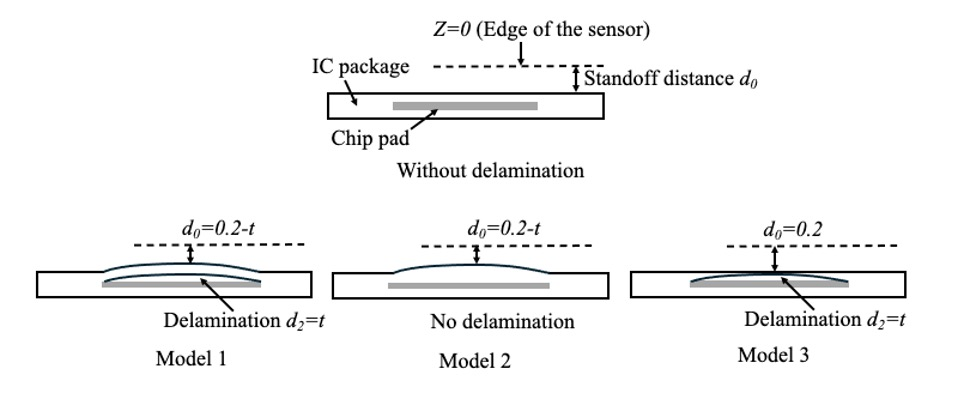
\includegraphics[width=0.8\linewidth]{Fig1.jpg}
    \caption{Delamination model of IC package: Model 1 assumes the standoff distance decreases with delamination (as in the dissertation's model), Model 2 assumes a reduced standoff distance without delamination, and Model 3 assumes a constant standoff distance with the presence of delamination.}
    \label{fig:delamination_model}
\end{figure*}

The results are summarized in Figure 
\ref{fig:phase_difference}.

\begin{figure*}[ht]
    \centering
    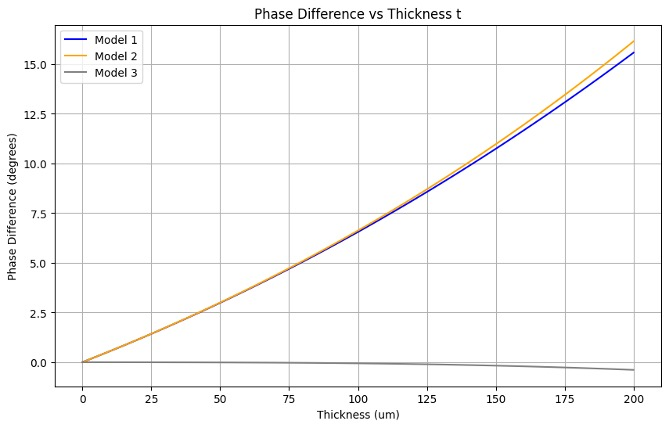
\includegraphics[width=0.8\linewidth]{Fig2.jpg}
    \caption{Phase difference of the effective reflection coefficient as a function of delamination thickness, calculated under three models.}
    \label{fig:phase_difference}
\end{figure*}

The key findings are:

\begin{itemize}
    \item \textbf{Model 1 and Model 2 produce nearly identical phase differences}, indicating that the primary effect is due to changes in \( t_0 \), not \( t_2 \).
    \item \textbf{Model 3 produces negligible phase variation}, suggesting that the direct influence of \( t_2 \) is much smaller than that of \( t_0 \).
    \item This implies that \textbf{the phase difference is dominated by variations in the standoff distance rather than the delamination thickness}.
\end{itemize}

Thus, the core assumption of the dissertation—that the phase difference reflects delamination thickness—is fundamentally flawed. Instead, the phase difference primarily measures how far the sensor is from the IC surface, rendering the method unreliable for delamination detection.

\subsection{Comparison with Existing Literature}

The dissertation cites Zoughi and Bakhtiari (1990) \cite{2} as a foundational study for its theoretical approach. However, there are significant differences between the two works:

\begin{itemize}
    \item \textbf{Scale Difference}: The Zoughi model was developed for millimeter-scale dielectric layers, whereas the dissertation applies it to micrometer delamination, which changes the sensitivity of the method.
    \item \textbf{Standoff Distance Consideration}: Zoughi’s model does not explicitly include standoff distance effects, as their setup used horn antennas rather than coaxial probes, which are more susceptible to positioning errors.
    \item \textbf{Empirical Validation}: Zoughi’s study included rigorous calibration and experimental validation, whereas the dissertation lacks sufficient experimental controls and validation steps.
\end{itemize}

Given these differences, it is questionable whether the Zoughi model can be directly applied to the dissertation’s context. This further weakens the dissertation’s claim that phase difference can be reliably used for delamination thickness measurement.


\section{Experimental Analysis}

The dissertation also presents experimental results that claim to validate the theoretical model. However, our re-examination of these experiments reveals significant methodological issues, including inadequate documentation of measurement conditions, potential selection bias in reported data, and lack of statistical validation. These issues call into question the reliability of the experimental findings.

\subsection{Overview of the Experimental Setup}

The dissertation describes a microwave measurement system consisting of:
\begin{itemize}
    \item A coaxial probe as the microwave sensor.
    \item A vector network analyzer (HP8510) for measuring the reflection coefficient.
    \item An automated scanning stage to move the IC package.
    \item A set of test samples with and without artificially introduced delamination.
\end{itemize}

The key experimental claim is that the phase difference of the reflection coefficient can be used to detect the presence and thickness of delamination within the IC package.

\subsection{Issues in Measurement Conditions and Sample Preparation}

Several critical issues regarding measurement conditions and sample preparation are either undocumented or inadequately addressed:

\begin{enumerate}
    \item \textbf{Lack of Control Over Standoff Distance:} As discussed in the theoretical analysis, the standoff distance \( t_0 \) has a dominant effect on the measured phase difference. However, the dissertation does not specify how \( t_0 \) was controlled, nor does it quantify the associated measurement uncertainty.
    \item \textbf{Limited Number of Test Samples:} The experimental results are based on only four IC samples (two with delamination, two without). Such a small sample size severely limits statistical reliability and raises concerns about the generalizability of the findings.
    \item \textbf{Artificially Introduced Delamination:} The dissertation states that delamination was introduced via controlled heating and moisture exposure, but it lacks details on the repeatability of this process. It remains unclear whether the artificially created delaminations accurately represent real-world defects.
    \item \textbf{Measurement Uncertainty and Equipment Calibration:} The dissertation does not provide calibration data for the network analyzer or discuss the expected accuracy of phase difference measurements.
\end{enumerate}

Given these omissions, the reliability of the reported results is highly questionable.

\subsection{Potential Selection Bias in Reported Data}

The dissertation does not specify how many experimental trials were conducted, nor does it present complete datasets. Instead, only selected measurement curves are shown, raising the possibility that results were chosen to fit the expected theoretical trend. Without full disclosure of all measured data, it is impossible to determine whether the presented findings are representative or selectively reported.

If multiple measurements were performed and only "good" results were included in the dissertation, this would constitute a significant methodological flaw, as it introduces confirmation bias. Scientific integrity requires transparency in reporting all collected data, including inconsistent or unexpected results.

\subsection{Lack of Statistical Validation}

The dissertation does not perform any statistical analysis to assess measurement reliability. Key statistical shortcomings include:

\begin{itemize}
    \item \textbf{Absence of Error Bars:} The reported phase difference measurements are presented as single curves without error margins, making it impossible to assess experimental variability.
    \item \textbf{No Repeatability Testing:} There is no indication that the same measurements were repeated multiple times to evaluate consistency.
    \item \textbf{No Hypothesis Testing:} The dissertation does not use statistical tests to confirm whether observed differences between delaminated and non-delaminated samples are significant.
\end{itemize}

Given the small sample size, lack of error analysis, and potential selection bias, the experimental claims in the dissertation do not meet the standards of rigorous scientific validation.

\subsection{Summary of Experimental Concerns}

In summary, the experimental analysis in the dissertation suffers from the following major flaws:

\begin{itemize}
    \item The dominant effect of standoff distance on phase difference was not accounted for.
    \item The number of test samples was too small to support meaningful conclusions.
    \item Measurement conditions, including standoff distance control and equipment calibration, were inadequately documented.
    \item Possible selection bias may have influenced the reported results.
    \item No statistical validation of the measurements was performed.
\end{itemize}

These deficiencies undermine the reliability of the dissertation’s experimental claims. Without addressing these issues, the conclusion that microwave phase difference can be used to evaluate IC package delamination remains unsubstantiated.

\section{Discussion}

The concerns raised in this study highlight fundamental issues in both the theoretical model and the experimental validation presented in the dissertation. These issues extend beyond a single research work and point to broader concerns regarding academic integrity, peer review, and doctoral dissertation evaluation processes.

\subsection{The Core Issue: What Was Actually Measured?}

The fundamental flaw in the dissertation is that the proposed microwave measurement method primarily detects variations in standoff distance rather than the thickness of the delamination layer. This contradicts the intended measurement target and fundamentally undermines the dissertation’s conclusions. 

If the phase difference of the reflection coefficient is primarily influenced by standoff distance rather than delamination thickness, then:
\begin{itemize}
    \item The dissertation does not actually provide a reliable method for measuring internal delamination.
    \item The experimental results are not direct evidence of delamination detection.
    \item Any correlation between measured phase difference and delamination thickness is incidental rather than causal.
\end{itemize}

This is not merely a minor error or oversight but a fundamental flaw in the measurement concept itself. A valid scientific method must ensure that the measured quantity corresponds to the intended physical phenomenon.

\subsection{Why Was This Not Identified During Dissertation Review?}

Given the fundamental nature of this issue, it is reasonable to ask why it was not identified during the dissertation review process. Three possible explanations exist:

\begin{enumerate}
    \item \textbf{Lack of Sufficient Expert Review:} The dissertation committee may not have included members with sufficient expertise in microwave nondestructive testing. Without proper scrutiny, a flawed model and its corresponding experimental results could have been mistakenly accepted.
    \item \textbf{Overreliance on Experimental Confirmation:} If reviewers focused on the experimental data without critically evaluating the theoretical basis, they may have accepted the conclusions without questioning whether the experiment truly measured delamination thickness.
    \item \textbf{Institutional Pressures:} Academic environments sometimes prioritize graduation rates and publication outputs over rigorous scientific scrutiny. If there was an implicit institutional pressure to approve dissertations without thorough review, this could have contributed to the oversight.
\end{enumerate}

This case serves as an example of how dissertation evaluation procedures may fail to catch fundamental errors, raising concerns about the robustness of doctoral examination standards.

\subsection{Potential Implications for the Field}

If the dissertation's conclusions were accepted without challenge, it is possible that subsequent research may have been misled by its claims. In applied fields such as microwave nondestructive testing, erroneous conclusions could lead to:
\begin{itemize}
    \item Misallocation of research resources toward ineffective measurement techniques.
    \item Incorrect industry applications based on unreliable methods.
    \item Further publications that build on a flawed theoretical foundation.
\end{itemize}

This demonstrates the importance of critically reviewing foundational studies to prevent the propagation of errors in scientific and engineering fields.

\subsection{Addressing These Issues: Ensuring Research Integrity}

To prevent similar issues in the future, institutions should strengthen the following aspects of dissertation evaluation:

\begin{itemize}
    \item \textbf{Ensuring Domain Expertise in Review Committees:} Dissertation committees should include experts with deep knowledge in the relevant field to rigorously assess theoretical models and experimental methodologies.
    \item \textbf{Requiring Transparent Data Disclosure:} Complete experimental datasets should be provided with doctoral dissertations to enable independent verification.
    \item \textbf{Encouraging Post-Publication Peer Review:} Mechanisms should be in place for researchers to raise concerns about published dissertations in a constructive academic setting.
\end{itemize}

These measures would help safeguard the reliability of scientific research and uphold the credibility of academic institutions.

\subsection{Summary of Discussion}

This case underscores the importance of rigorous theoretical and experimental validation in scientific research. The primary concerns identified in the dissertation include:
\begin{itemize}
    \item The theoretical model does not support the claimed measurement of delamination thickness.
    \item Experimental data selection and reporting lack transparency.
    \item The dissertation review process failed to identify these fundamental flaws.
\end{itemize}

While individual errors in research are inevitable, doctoral dissertations represent the culmination of a researcher’s academic training and must be held to the highest standards. This case serves as a cautionary example of the consequences when such standards are not met.

\section{Conclusion}

This study critically re-examined the theoretical and experimental framework of the doctoral dissertation by Ju Yang, which proposed a microwave nondestructive evaluation method for detecting delamination in IC packages. Through a detailed analysis, we identified significant issues in both the theoretical model and the experimental validation, raising concerns about the validity of the dissertation’s conclusions.

\subsection{Key Findings}

The primary findings of this study are as follows:

\begin{itemize}
    \item \textbf{Fundamental Measurement Issue:} The theoretical model suggests that the phase difference of the reflection coefficient is more strongly influenced by standoff distance than by delamination thickness. This implies that the proposed method does not directly measure delamination, fundamentally undermining its claims.
    \item \textbf{Experimental Transparency and Reproducibility:} The dissertation lacks essential details regarding experimental conditions, including the number of test samples, statistical treatment of the data, and explicit methodologies for controlling standoff distance. This raises concerns about the reliability and reproducibility of the reported results.
    \item \textbf{Doctoral Dissertation Review Process:} The acceptance of this dissertation despite its fundamental theoretical flaws and experimental shortcomings suggests potential weaknesses in the dissertation evaluation process, highlighting the need for more rigorous academic scrutiny.
\end{itemize}

\subsection{Implications for Research Integrity}

This case underscores broader issues in academic research integrity. If doctoral dissertations are not subjected to rigorous theoretical and experimental validation, the credibility of academic institutions and the reliability of published research come into question. Key implications include:

\begin{itemize}
    \item The necessity of ensuring that theoretical models align with experimental objectives in applied scientific research.
    \item The importance of transparent and reproducible experimental methodologies.
    \item The need for dissertation committees to include domain experts capable of critically assessing both theoretical and empirical aspects.
    \item The value of post-publication peer review mechanisms to address potential research deficiencies.
\end{itemize}

\subsection{Future Directions}

Addressing these issues requires a multi-faceted approach. We propose the following actions:

\begin{itemize}
    \item \textbf{Institutional Improvements:} Universities should strengthen dissertation review processes by mandating independent verification of theoretical models and experimental methods.
    \item \textbf{Encouraging Open Scientific Debate:} Mechanisms should be in place to allow for post-publication scrutiny and correction of research errors without reputational risks to whistleblowers.
    \item \textbf{Enhancing Research Ethics Education:} Graduate programs should emphasize the importance of methodological rigor, transparent reporting, and ethical research practices.
\end{itemize}

\subsection{Final Remarks}

The case examined in this study serves as a cautionary example of how unchallenged assumptions, lack of methodological rigor, and inadequate peer review can lead to flawed research being accepted at the highest academic level. While errors in scientific research are inevitable, the processes designed to prevent them—rigorous theoretical examination, transparent experimental validation, and robust peer review—must function effectively to uphold the integrity of the academic enterprise.

The acceptance of a dissertation with such fundamental flaws calls for a reassessment of academic standards in doctoral education and research evaluation. It is our hope that this case prompts further discussion and institutional reforms to strengthen research integrity and ensure that doctoral dissertations meet the highest scientific standards.


$\,$

$\,$

\begin{thebibliography}{99}

\bibitem{1} Ju, Yang, "A Study on Microwave Nondestructive Evaluation of Delamination in IC Package", Doctoral Dissertation, Tohoku University, 1999.

\bibitem{2} Zoughi, R. and Bakhtiari, S., "Microwave Nondestructive Detection and Evaluation of Disbonding and Delamination in Layered-Dielectric-Slabs", IEEE Transactions on Instrumentation and Measurement, Vol. 39, No. 6, 1990, pp. 1059-1063.

\end{thebibliography}
\end{document} 